% !TEX program = xelatex

\documentclass{beamer}
\usepackage[utf8]{inputenc}
\usepackage{xeCJK}
\usepackage{utopia} %font utopia imported
%\usepackage[UTF8,noindent]{ctexcap}
\usepackage{latexsym,amssymb,amsmath,amsbsy,amsopn,amstext,xcolor,multicol}
\usepackage{graphicx,wrapfig,fancybox}
% \usetheme{Rochester}
\usetheme{Madrid}
\usecolortheme{default}
 % 衬线字体:Linux Libertine
    % BoldFont 可以选择 Bold 字重或者 Semibold 字重
    % BoldItalicFont 也有对应 BoldFont 的字重选择
    % 这里使用 Semibold 字重
  %   \setmainfont{LinLibertine_R.otf}[
  %     BoldFont = LinLibertine_RZ.otf,
  %     ItalicFont = LinLibertine_RI.otf,
  %     BoldItalicFont = LinLibertine_RZI.otf]
  % % % 无衬线字体:Linux Biolinum
  % \setsansfont{LinBiolinum_R.otf}[
  %     BoldFont = LinBiolinum_RB.otf,
  %     ItalicFont = LinBiolinum_RI.otf,
  %     BoldItalicFont = LinBiolinum_RBO.otf]
  % % 等宽/打印机字体:Linux Libertine Mono
  % \setmonofont{LinLibertine_M.otf}[
  %     BoldFont = LinLibertine_MB.otf,
  %     ItalicFont = LinLibertine_MO.otf,
  %     BoldItalicFont  = LinLibertine_MBO.otf]
  % \setCJKmainfont[ItalicFont={AR PL UKai CN},
  % BoldFont={WenQuanYi Micro Hei}]{IPAMinCho,IPA明朝}
  \setCJKsansfont{WenQuanYi Micro Hei}
  \setCJKmonofont{WenQuanYi Micro Hei Mono}
%------------------------------------------------------------
%This block of code defines the information to appear in the
%Title page
\title[光电报告] %optional
{光电子技术实验}

\subtitle{波长检测型表面等离子体共振 (SPR) 传感}

\author[芦, 王] % (optional)
{芦迪 \and 王莘景}

\institute[THU, EE] % (optional)
{
  Department of Electronic Engineering,\\
  Tsinghua University
}

\date[2017.11.29] % (optional)
{November 29, 2017}

\logo{
\includegraphics[height=1.5cm]{images/thuee-logo.png}}

%End of title page configuration block
%------------------------------------------------------------



%------------------------------------------------------------
%The next block of commands puts the table of contents at the 
%beginning of each section and highlights the current section:

\AtBeginSection[]
{
  \begin{frame}
    \frametitle{目录}
    \tableofcontents[currentsection]
  \end{frame}
}
%------------------------------------------------------------


\begin{document}
%The next statement creates the title page.
\frame{\titlepage}


%---------------------------------------------------------
%This block of code is for the table of contents after
%the title page
\begin{frame}
\frametitle{目录}
\tableofcontents
\end{frame}
%---------------------------------------------------------


\section{实验任务}

%---------------------------------------------------------
%Changing visivility of the text
\begin{frame}{实验任务}
  本次实验的实验目的为:
  \begin{enumerate}
    \item 了解表面等离子体共振(SPR)波长检测原理
    \item 了解实现波长检测表面等离子体共振检测的系统结构
    \item 结合理论分析结果,探索研究影响系统检测性能的各项因素
  \end{enumerate}
  \
  
  \pause
  为达到以上目的,实验设计了如下任务:
  \begin{enumerate}
      \item 利用波长调整型 SPR 传感系统对纯水、苏打水和食盐水等物质进行检测,得到检测光谱
      \item 探索研究入射光角度、偏振态、金膜厚度等因素对检测光谱特性的影响
  \end{enumerate}
\end{frame}

%---------------------------------------------------------


%---------------------------------------------------------
%Example of the \pause command
% \begin{frame}
%   \frametitle{实验原理}
% In this slide \pause

% the text will be partially visible \pause

% And finally everything will be there
% \end{frame}
%---------------------------------------------------------

\section{实验原理}

%---------------------------------------------------------
%Highlighting text
\begin{frame}{检测原理}
% \frametitle
\begin{itemize}
  \item 表面等离子体共振(简称SPR)是一种物理光学现象,利用光在玻璃界面处发生全内反射时的消逝波,激发出沿金属薄膜表面传播的表面等离子体波(SPW)
  \item 在入射角或波长为某一适当值的条件下,入射光与 SPW 发生共振,此时全反射的反射光能量急剧下降,在反射光谱上出现共振吸收峰
\end{itemize}
\begin{figure}
  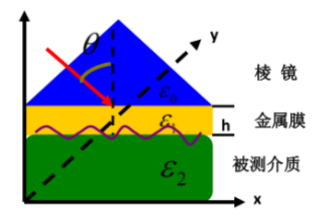
\includegraphics[height=2.86cm,width=4.29cm]{images/2_2.png}
  \caption{棱镜型 SPR 传感器结构}
\end{figure}
\end{frame}
\begin{frame}{检测原理}
  \begin{itemize}
    \item 当紧靠在金属薄膜表面的介质折射率不同时, 共振峰位置将不同
    \item SPR 的共振峰位置与被测介质的性质密切相关, 根据对这个信号的检测就可以获得被测物质的折射率、浓度、膜层厚度、反应进程等信息, 从而达到生化检测的目的
  \end{itemize}
  \begin{figure}
    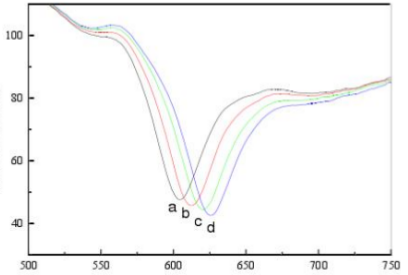
\includegraphics[height=3.575cm,width=5.304cm]{images/2_1.png}
    \caption{波长调制检测方法对不同物质检测的仿真结果}
  \end{figure}
\end{frame}

%---------------------------------------------------------
% 
%---------------------------------------------------------

\section{理论仿真}
\begin{frame}{理论仿真}
  利用MATLAB软件对波长检测型SPR传感结果进行仿真,并研究了实验条件对检测结果的影响,用以对实验条件建设提供理论依据。结论如下:
  \begin{enumerate}
    \item 当被测物质一定时,入射角变小,共振波长变大,共振半峰宽度变大,共振深度增大灵敏度变大。
    \item 当入射角度不变时,被测物质折射率增大,共振波长变大,共振半峰宽度变大,共振深度增大,灵敏度变大。
    \item 存在一个合适大小的金属膜厚度使得实验效果最好,反射率最低点最低吸收效果最好而且半峰宽较窄。本次仿真中的最佳结果为 50nm,当厚度小于 50 时半峰宽较大而且吸收峰的共振深度较小;当厚度大于 50nm 时半峰宽降低但是吸收峰共振深度也减小。
    \item 入射角度的改变会使得被测物质的检测范围发生改变。入射角度变大,检测范围变大,检测灵敏度变小。
  \end{enumerate}
  
\end{frame}

\section{实验系统}
\begin{frame}{实验系统}
  \begin{itemize}
    \item 实验所用SPR检测系统依据Kretchsmann棱镜型结构和波长调制原理搭建,主体结构为:
    \begin{figure}
      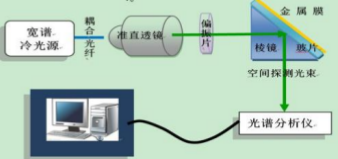
\includegraphics[height=3.29cm,width=7cm]{images/2_3.png}
    \end{figure}
  \end{itemize}
  

% \begin{block}{装置简述}
%   \begin{description}

%   \end{description}
% \end{block}
  
\end{frame}


\section{方法步骤}
\begin{frame}{光路调整}
  \begin{itemize}
    \item 入射角调到自己需要的角度,这里就可以根据发射机上的角度刻度值实现
    \item 可以调节棱镜和发射机的高度使得传感区位于棱镜底部的中心位置,这一步我们可以使用擦镜纸在棱镜两侧相同距离处观察光斑的垂直位置,基本保证两个光斑在同一竖直高度即可
    \item 打开电脑光谱仪,接收棱镜反射回来的光,调整接收机使得收到的光谱尽量的大,这一步是实验中最困难的,我们要确保光线与接收机同轴,我们用擦镜纸在接收机接收处可以发现两个光斑,一个是棱镜反射传过来的,一个是接收机后光纤端面反射过来的,我们应调整接收机角度、高度,使得这两个光斑尽量重合与接收面中心处。如果觉得调整的比较理想但还是没有光谱就可以看着光谱微调
  \end{itemize}
\end{frame}
\begin{frame}{放置金片}
  \begin{enumerate}
    \item 注意清洁,先滴匹配油,再用镊子将金片放置在棱镜上,需要注意的是金片的正反面,用镊子轻轻划擦,能够看到痕迹的就是镀有金膜的一面,该面朝上即可
  \end{enumerate}
\end{frame}
\begin{frame}{滴加液体}
\begin{block}{注意}
  \begin{itemize}
    \item 将不滴液体时的光谱设置为参考光谱,滴加液体时需要注意不要滴加太多液体,只要让使液体覆盖传感区,即棱镜中心位置就可以了。再换液体时需要使用吸水纸吸掉液体,注意使用吸水纸时,尽量不要在水平方向用力,避免摩擦损坏金膜,此外还要注意滴加液体时使用移液枪实现
  \end{itemize}
\end{block}
\end{frame}
\begin{frame}{测量折射率}
    \begin{itemize}
      \item 用实验室的仪器测量,在老师的帮助下也是掌握了测量方法,测得了我们需要的数据
    \end{itemize}
  \end{frame}


\section{实验结果及分析}

\begin{frame}{静态激光器输入输出关系曲线}
  \begin{itemize}
    \item 对实验测量得到的数据进行整理后,绘制出静态激光器输入输出关系曲线如下:
    \begin{figure}
      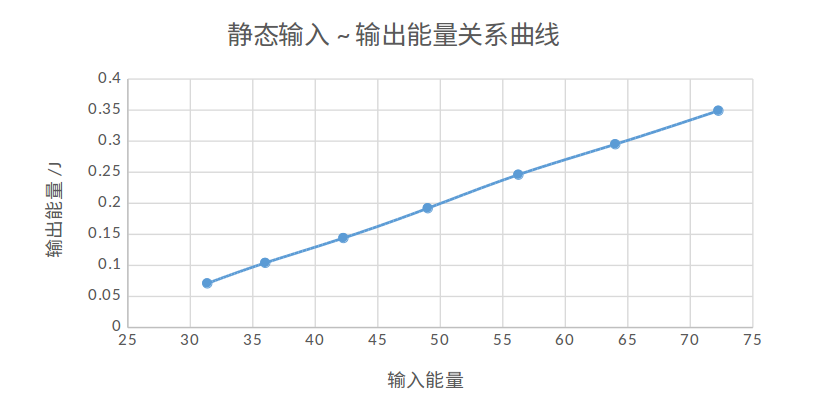
\includegraphics[height=4cm,width=8cm]{images/7.png}
      \label{fg7}
    \end{figure}
    \item 对于静态固体激光器,输出能量与输入能量近似线性变化。这表明当激光器在这一区间工作时,输出能量与输入能量成线性关系。
  \end{itemize}
\end{frame}

\begin{frame}{固体激光器静态输出波形}
  \begin{itemize}
    \item 取输入电压为700V,通过示波器观察驰豫振荡波形并测量其脉冲宽度,实验结果如下:
    \begin{figure}
      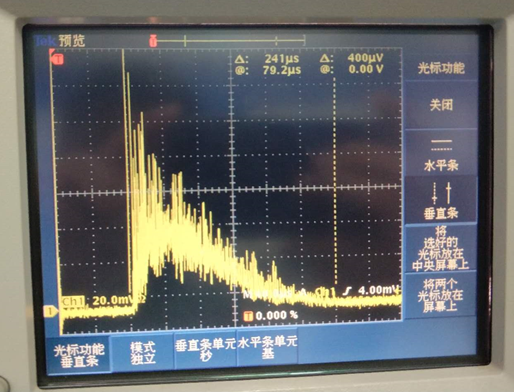
\includegraphics[height=3.92cm,width=5.14cm]{images/8.png}
      \label{fg7}
    \end{figure}
    \item 可以看到确实产生了驰豫振荡,脉冲宽度利用手动光标测量测得约为\(241\mu s\),符合我们的预期。
  \end{itemize}
\end{frame}
\begin{frame}{调Q激光器输入输出能量关系曲线}
  \begin{itemize}
    \item 加入调Q晶体后,我们按照之前的方法重新测量了阈值,得到阈值约为670V,较之前相比有所提高。整理得到的数据,绘制出调Q激光器输入输出关系曲线如下:
    \begin{figure}
      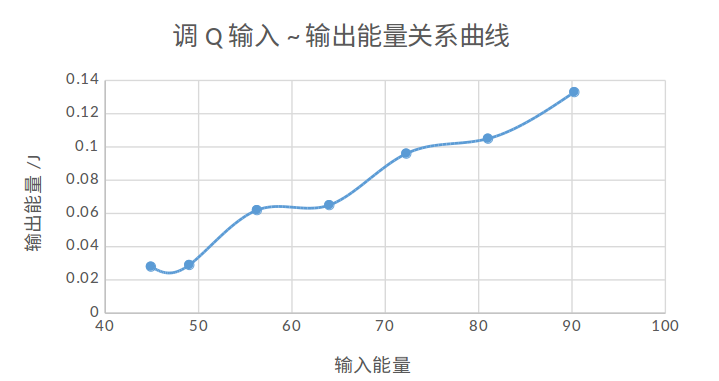
\includegraphics[height=3.8cm,width=7.2cm]{images/9.png}
      \label{fg7}
    \end{figure}
    \item 调Q时输入输出能量关系不再为线性,而是一种类似于阶梯的关系,与我们的理论推算相符。但可能图像采样点太少,阶梯不是太明显。
  \end{itemize}
\end{frame}


\begin{frame}{固体激光器调Q输出波形}
  \begin{itemize}
    \item 添加调Q晶体后,改变输入电压并通过示波器测得此时的输出波形,同时观测脉冲个数,观测结果:
    \begin{figure}[htbp]
      \centering
      \begin{minipage}[htbp]{80pt}
        \centering
        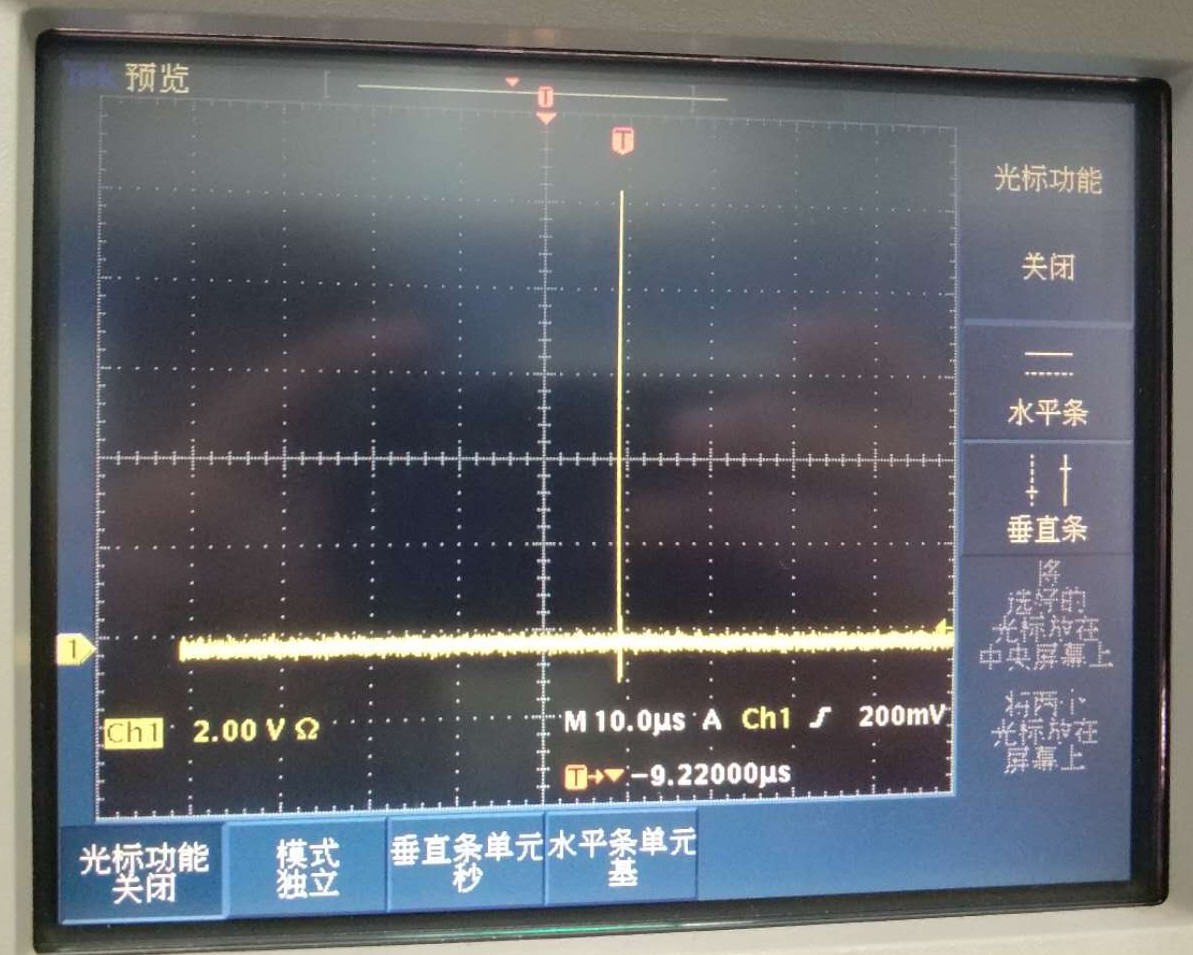
\includegraphics[width=80pt]{images/10.jpg}
        \caption{700V}
        \label{fig:4}
      \end{minipage}
      \hspace{10pt}%
      \begin{minipage}[htpb]{80pt}
        \centering
        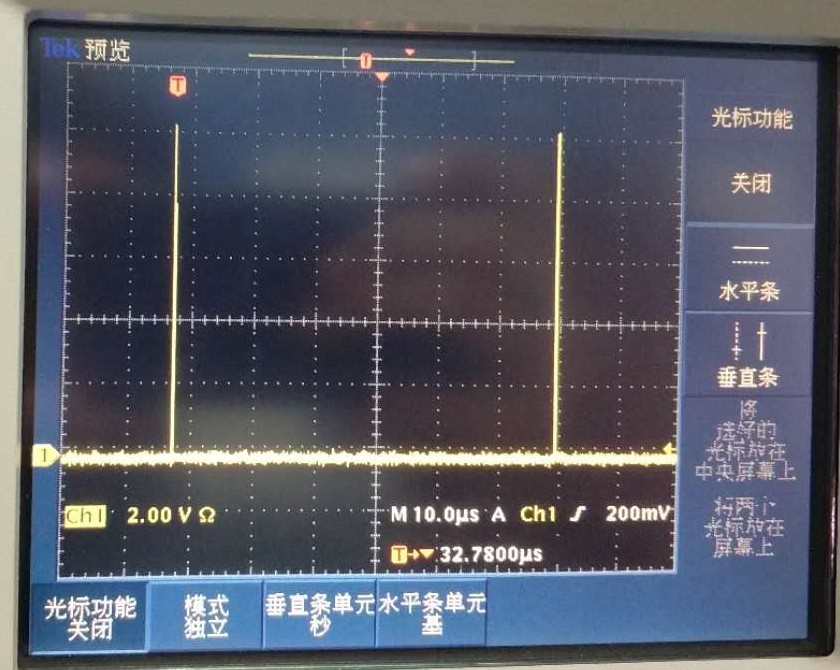
\includegraphics[width=80pt]{images/11.jpg}
        \caption{750V}
        \label{fig:5}
      \end{minipage}
      \hspace{10pt}%
      \begin{minipage}[htpb]{80pt}
        \centering
        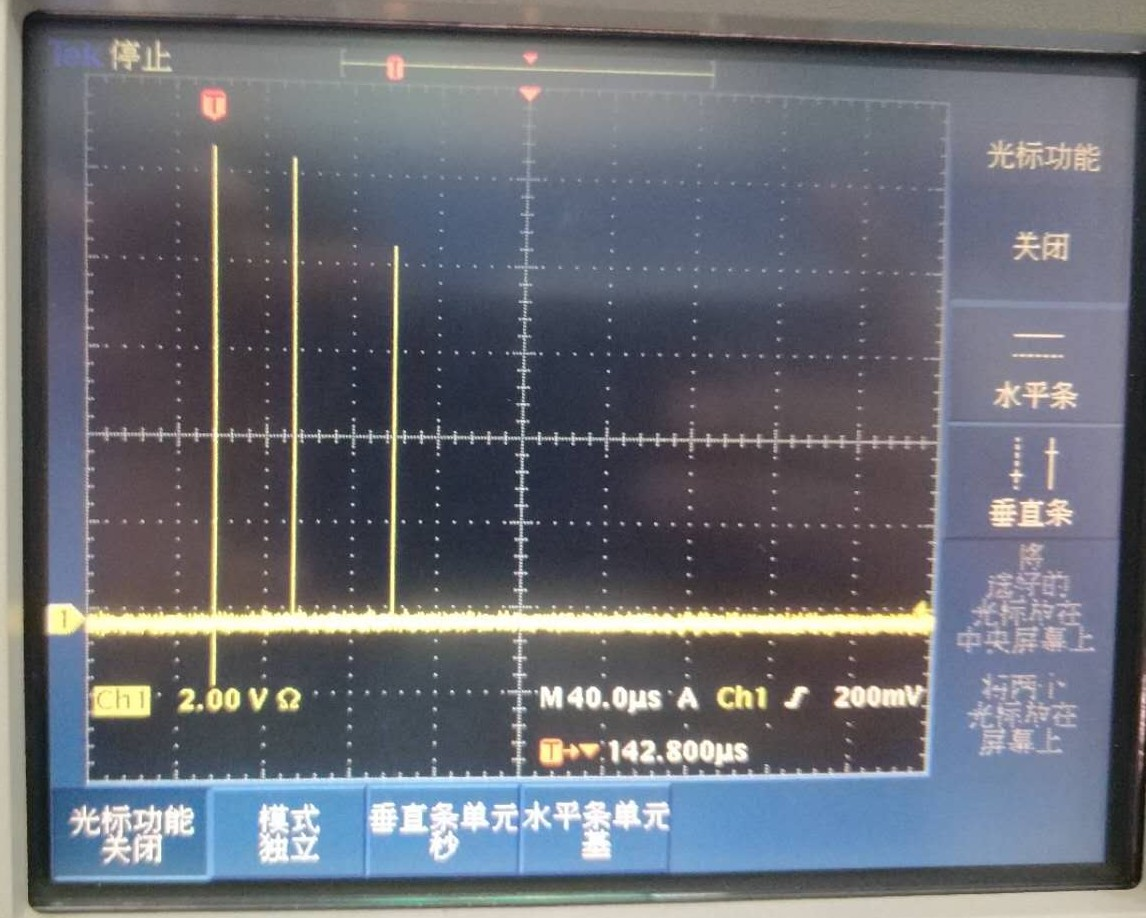
\includegraphics[width=80pt]{images/12.jpg}
        \caption{850V}
        \label{fig:5}
      \end{minipage}
      \end{figure}
    \item 随着输入电压增加,脉冲个数会呈阶梯状提高,应证了我们上一步得到的阶梯曲线。
  \end{itemize}
\end{frame}

\begin{frame}{调Q激光器输入输出能量关系曲线}
  \begin{itemize}
    \item 将 700V时的波形在脉冲处展开,得到的更加细致的波形为:
    \begin{figure}
      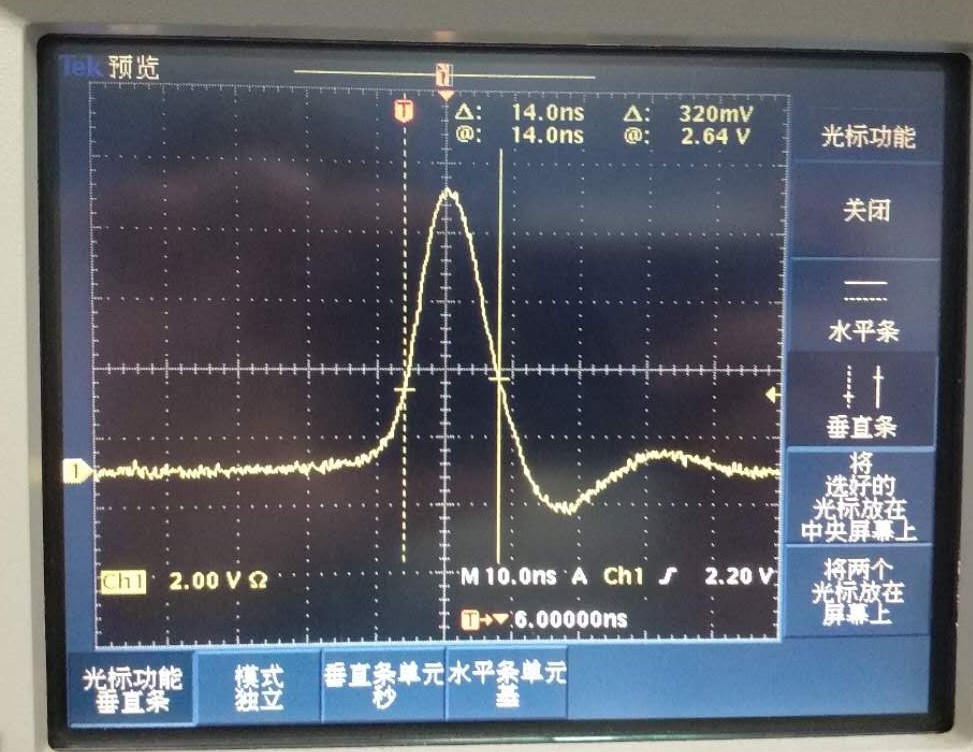
\includegraphics[height=4cm,width=5cm]{images/13.jpg}
      \label{fg7}
    \end{figure}
    \item 调整横纵坐标尺度使得脉冲尽量展开,然后利用手动测量测得单脉冲波形半高全宽约为14ns,符合我们的理论预期
  \end{itemize}
\end{frame}
\begin{frame}{谐振腔调制精度对激光器性能的影响}
  \begin{itemize}
    \item 调偏全反膜,通过目测望远镜视野中叉丝偏离的距离来表示角度偏离,取电压为700V,将得到的数据绘制为曲线:
    \begin{figure}
      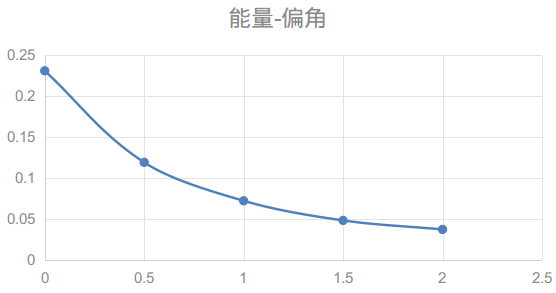
\includegraphics[height=3cm,width=5.5cm]{images/14.png}
      \label{fg7}
    \end{figure}
    \item 在固定输入能量的情况下,随着谐振腔的偏差,输出能量衰减,且开始时衰减得更剧烈。由于我们取的步长太大,这里并没有表现出微调时的结果。
  \end{itemize}
\end{frame}


\begin{frame}
    \begin{figure}
      
\includegraphics[height=2.23cm,width=4.29cm]{images/thank.jpg}
      \label{fg7}
    \end{figure}
   
\end{frame}
\end{document}


% In this slide, some important text will be
% \alert{highlighted} beause it's important.
% Please, don't abuse it.

% \begin{block}{Remark}
% Sample text
% \end{block}

% \begin{alertblock}{Important theorem}
% Sample text in red box
% \end{alertblock}

% \begin{examples}
% Sample text in green box. "Examples" is fixed as block title.
% \end{examples}

%---------------------------------------------------------
%Two columns
% \begin{frame}
% \frametitle{Two-column slide}

% \begin{columns}

% \column{0.5\textwidth}
% This is a text in first column.
% $$E=mc^2$$
% \begin{itemize}
% \item First item
% \item Second item
% \end{itemize}

% \column{0.5\textwidth}
% This text will be in the second column
% and on a second tought this is a nice looking
% layout in some cases.
% \end{columns}
% \end{frame}